%%
%% Author: thompson
%% 03.11.17
%%

% Preamble
\documentclass[11pt]{article}

% Packages
\usepackage{a4wide}
\usepackage[ngerman]{babel}
\usepackage[utf8]{inputenc}

\usepackage{scrextend}
\usepackage{enumerate}
\usepackage{graphicx}

% Document
\begin{document}
    \section{Analysis mit Wireshark}
    Im Rahmen folgender Fragestellungen analysieren wir mithilfe von Wireshark das beiliegende dump\_protocols.pcap.
    \begin{enumerate}[\thesection .1]
        \item Welche Netzwerkprotokolle werden in der Kommunikation verwendet?\\
        Es lassen sich mehrere Protokolle identifizieren, mitunter:
        \begin{addmargin}[1em]{1em}
            $\diamond$ DHCP - Dynamic Host Configuration Protocol: Zuweisung von Client \& Server.\\
            $\diamond$ ARP - Address Resolution Protocol: Zuweisung der MAC-Adressen im Lokalen Netzwerk.\\
            $\diamond$ ICMP - Internet Control Message Protocol: Handling von Fehler und Status in IP/TCP/UDP\\
            $\diamond$ DNS - Domain Name System: Zuweisung von IPs und Hostnamen.\\
            $\diamond$ TCP - Transmission Control Protocol: Datenübertragungsprotokoll, orientiert an sicherer Packetzustellung.\\
            $\diamond$ HTTP - HyperText Transfer Protocol: User Agent-Rendering gemäß .htmls\\
        \end{addmargin}

        \item Ordnen Sie jedes der Protokolle einer Schicht im TCP/IP-Referenzmodell zu und stellen Sie die Hierarchie der einzelnen Protokolle graphisch dar.\\
        Zunächst eine Wiederholung des TCP-IP Schichtenmodelles:
        \begin{center}
            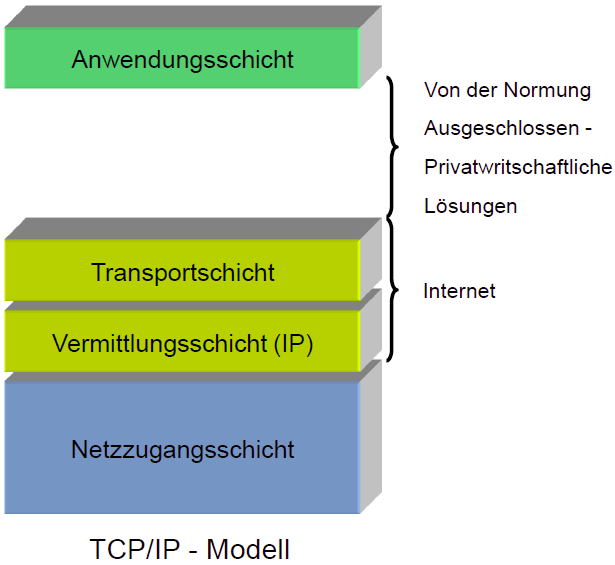
\includegraphics[width=30em,height=30em]{TCP-IP-Modell.png}
        \end{center}
\pagebreak
        Die genutzten Protokolle stehen somit in Folgender Relation zum TCP-IP Modell:
        \begin{addmargin}[1em]{1em}
            $\circ$ DHCP - Application Layer, als auch für das OSI-Model\\
            \emph{Grund}: DHCP vermittelt eine Client-Server verbindung basierend auf dem ausgeführtem Programm.
            Gibt es kein Programm, so gibt es weder spezifizierten Klienten noch Server.\\\\
            $\circ$ ARP - Network Access Layer, or Data Link Layer for the OSI-Model\\
            \emph{Grund}: ARP befasst sich mit der Korrektheit der MAC-Adressen. Diese befinden sich im Datalink Layer (OSI) und somit
            im Network Access Layer des TCP-IP.\\\\
            $\circ$ ICMP - Vermittlungsschicht, or Network Layer für OSI\\
            \emph{Grund}: ICMPvX beschäftigt sich mit Fehlercodes des IPvX, weshalb es keinem anderen Layer zuschreibbar ist als dem Network-Layer des OSI-Models.
            Dementsprechend befindet es sich in der Vermittlungsschicht.\\\\
            $\circ$ DNS - Application Layer - parallel mit HTTP, eben so für das OSI-Model\\
            \emph{Grund}: DNS beschäftigt sich mit dem Zuschreiben von Aliasen der IP-Adressen, den Hostnamen.
            Dieser findet jedoch nur im Browser(=Applikationsschicht) nutzen, da aus maschineller Sicht die Hostnamen IP-Adressen wiederspiegeln.\\\\
            $\circ$ TCP - Transport Layer für das TCP-IP als auch OSI-Model\\
            \emph{Grund}: TCP beschäftigt sich mit dem Datenaustausch über Handshake. Als bekanntes Protokoll dient es der sicheren Übertragung von Frames
            und ist dementsprechend auf dem Transportlayer angesiedelt.\\\\
            $\circ$ HTTP - Application Layer, ebenso für OSI\\
            \emph{Grund}: HTTP dient der Übertragung der spezifizierten .htmls eines Servers, gewöhnlicherweise via TCP/IP.
            Da HTML (\& css sowie js oder php, etc.) der Darstellung einer Seite dienen, gilt HTTP der Applikationsschicht.
        \end{addmargin}
\pagebreak
        Graphisch wären die Protokolle etwa so einzugliedern:\\
        \begin{center}
            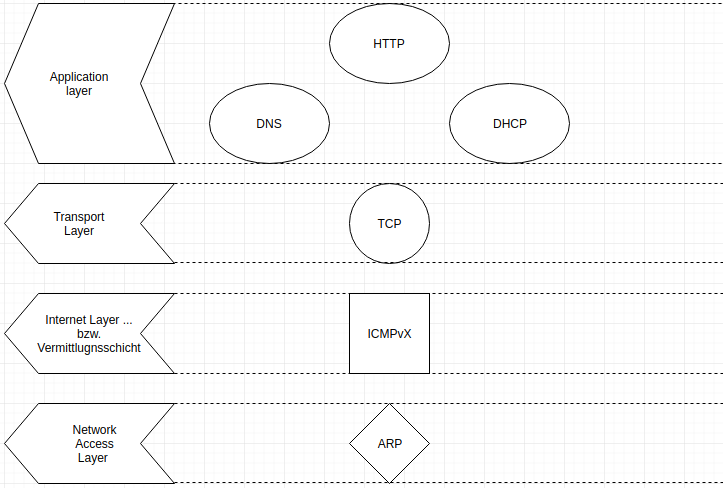
\includegraphics[width=\textwidth]{Modelization.png}
        \end{center}
        Alternativ:
        \begin{verbatim}
            Statistics > Protocol Hierarchy
        \end{verbatim}
    \end{enumerate}
\end{document}